%!TEX root = ../main.tex
\chapter{Methodology}\label{chapter:methodology}
In this chapter we will give overview of our system design and work flow.
First, we will give short technical descriptions of terms we will be using to describe our work flow in~\autoref{sec:Terminology}
We will look upon the overall procedure and also discuss on why we chose certain approach in~\autoref{sec:Work Flow}.
Let us start with the overview of our experiment.
\section{Terminology}
\label{sec:Terminology}
In this section we give a detailed description of different terms we will be using through out the report.
\subsection{Behavioral Profile}
\label{sub:Behavioral Profile}
According to the authors,~\citeauthor{bayer}, ``\textbf{behavioral profile}'', is defined as, ``the abstraction of a program's execution trace that provides information on the OS objects that the program operated on, along with the operations''.
OS Object refers to resource type such as file, registry or section, that could be modified or queried with the system calls.
System calls consisted of Windows NT, native API and the Windows API functions.\\
The behavioral profile was based on the execution traces of programs irrespective of order execution as reordering system calls could be done without changing the semantics of program~\cite[]{bayer}.
It consisted of a list of different operations operated on the different OS objects during the execution of binary.
The system calls that had same purpose as resultant output but different calling API name were generalized under single name--\emph{NtCreateProcess} and \emph{NtCreateProcessEx} would be generalized as, \emph{`create'} OS Operation for, \emph{`porcess'} OS object~\cite[]{bayer}.\\
\subsubsection{OS Objects}
\label{ssub:OS Objects}
OS Object were primarily the resource that were created, delete, modified during the program execution.
\citeauthor{bayer} define \emph{OS Objects} as:
\begin{lstlisting}
OS Object ::= (type, object-name)
type ::= file|registry|process|job|
       network|thread|section|
       driver|sync|service|random|
       time|info
\end{lstlisting}
An OS Object consists of its type and object-name.
The type of OS Object are file, registry, process, job, network, thread, section, driver, sync, service, random, time, and info.
An object-name is the name of the OS object.
For an instance, \url{`c:\\ntlos.exe'} is an object-name for object type \emph{file}.

\subsubsection{OS Operations}
\label{ssub:OS Operations}
Broadly, OS Operation is the generalization of a system call.
\citeauthor{bayer} define \emph{OS Operations} as:
\begin{lstlisting}
OS operation ::= (operation-name,
                opeartion-attributes?,
                successful?)
\end{lstlisting}
An OS operation object consists of name of the operation, any additional attributes, and the status of the operation whether it was successful or not.\\
A snippet of behavioral profile is shown in~\autoref{lst:bpsample} with sample of operations executed on OS Objects file, registry, and section.
\begin{lstlisting}[language=TeX,caption={Behvaioral Profile sample}, label={lst:bpsample}]
  op|file|`C:\\Program Files\\Common Files\\sumbh.exe'
   create:1
   open:1
   query:1
   write:1

  op|registry|`HKLM\\SOFTWARE\\CLASSES\\CLSID\\{00021401-0000-0000-C000-000000000046}'
   open:1
   query:1
   query_value(''):1
   query_value('ThreadingModel'):1

  op|section|`BaseNamedObjects\\MSCTF.MarshalInterface.FileMap.ELE.B.FLKMG'
   create:1
   map:1
   mem_read:1
   mem_write:1
\end{lstlisting}
To explain the behavioral profile in~\autoref{lst:bpsample}, \textit{`create'} operation for file OS object \url{`C:\\Program Files\\Common Files\\sumbh.exe'} was successful with success value 1, whereas \textit{`query\_value'} operation with operation-attribute value \emph{'InprocServer32'} for registry OS Object \url{`HKLM\\SOFTWARE\\CLASSES\\CLSID\\{00021401-0000-0000-C000-000000000046}'} failed with success value 0. % chktex-file 8
\\

We used the behavioral profiles of the malware sample to recreate new database, as per our research need, which is described in~\autoref{sec:Creation of Database}.
Our interest were list of \emph{OS Objects} and \emph{Operations} associated with the behavioral profile of the malware.
We used those information to recreate the database of all the malware (program) samples and its resource activities (execution traces).
\subsection{Resource Type and Activities}
\label{sub:Resource Types and Activities}
As discussed before in~\autoref{ssub:OS Objects}, an OS Object, are representation of resource types.
For our research, we took into consideration following 8 resource types among those list, that could best determine the behavioral interference between malware.
We will give a short description of each resource type according to Microsoft Developers Network documentation~\cite[MSDN]{msdn}.
\subsubsection{File}
\label{ssub:File}
A \emph{file} is a means of storing resourceful information which can be retrieved or modified in future.
File objects function as the logical interface between kernel and user-mode processes and the file data that resides on the physical disk.
It not only holds the data written on the file but also a set of attributes maintained by the kernel for system purposes such as \emph{File name, Current byte offset, Share mode, I/O mode}~\cite[]{msfile}.\\
File type in the behavioral profile encompasses not only general file, but named pipe and mailslot resources.
% File is an important resource type for us to focus as our hypothesis for research is that malware of certain family creates or deletes a certain file to infect a system and this also could be used by malware of another family to remove its nemesis from system.
File is an important resource type as many malware creates or deletes file in order to infect the system or remove another malware from the system.
These file activities will be important behavior to find the interference between malware families.
\subsubsection{Registry}
\label{ssub:Registry}
A \emph{Registry} is a database defined by a system where different applications and system components store and retrieve data such as configurations settings for its use.
The data stored in the registry varies according to the version of Microsoft Windows.
Application performs the basic add, modify, retrieve, or delete operation in the registry through the registry API~\cite[]{msregistry}.\\
% We take the registry keys associated with the malware into consideration for experiment as it provides vital information on the behavior of a malware sample.
% Malware with same family might have similar registry key activity and also malware from different family might look for the particular registry key in the system in order to detect the presence of another family.
Registry keys provide vital information on malware type and behavior.
We have seen in~\autoref{sec:Malware Families} that different malware families create different registry keys when they infect a system.
\subsubsection{Service}
\label{ssub:Service}
A \emph{Service} is a computer program that operates in system background, similar to UNIX daemon~\cite[]{servicedef}.
A \emph{service} can be started at system boot through the Service Control Panel, or an application can also use service functions such as \emph{StartService, OpenService, DeleteService} to configure services.
However, it must conform to the interface rules of Service Control Manager (SCM)~\cite[]{msservice}.\\
Malware can stop other services related to security or other malware, create a new service, or hook itself into autostart services.
These service related activity are interesting to study malware behavior and interaction with other malware.
\subsubsection{Section}
\label{ssub:Section}
A \emph{section} object is sharable memory which is used by process to share its memory address space (memory sections) with other processes.
It is also used by process to map a file into its memory address space~\cite[]{mssection}.\\
In case of behavioral profile, it broadly represents memory mapped files.
\subsubsection{Process}
\label{ssub:Process}
A binary can spawn one or more \emph{processes}.
A process is simply an instance of a computer program being executed that consists of instructions and current activity of program.
One or more threads can be run in the context of the process~\cite[]{msprocess}.\\
Malware constantly look for creation of new process such as \emph{Task Manager} or \emph{Virus Removal Tools} and shuts it down before it starts.
Similar behavior in case of process created by other malware will be a proof for behavioral interference between malware families.
\subsubsection{Job}
\label{ssub:Job}
A \emph{Job} object makes grouping of process as single unit to manage possible.
It can be named and shared securely to control attributes of processes grouped together and operation on a job makes the affect on all the process in its group~\cite[]{msjob}.
\subsubsection{Sync}
\label{ssub:Sync}
A \emph{sync object} is used to coordinate the execution of multiple threads as more than one process could share the handle of single synchronization object which helps for the interprocess synchronization between these processes~\cite[]{mssync}.\\
The sync object type covers all the synchronization activities.
\cite[]{mssync}.
\subsubsection{Driver}
\label{ssub:Driver}
A \emph{device driver } is a program that is associated with certain device for its operation and control. It is used as an software interface to communicate between the hardware device and the operating system and other software~\cite[Device Driver]{devicedriver} \\
Windows represent devices with device objects, and one device could be represented by more than one device objects. All operation on device is conducted via device object~\cite[]{msdevice}.\\
We capture those loading and unloading of Windows Device Driver recorded in the behavioral profile.\\

\textbf{Resource activities} in our work refers to operations, such as \emph{create, delete, modify, or access}, performed by a malware (program), on the resource types \emph{File, Registry, Service, Section, Process, Job, Sync, or Driver}, during its execution.
\textbf{Resource name} is same as object-name in \emph{OS-Objects}[\autoref{ssub:OS Objects}] -- name of the resource created, modified, deleted, or accessed.
We use resource activities of malware samples to select the malware candidates that could exhibit behavioral interference [\autoref{sec:Initial Experiment}].
Further, resource activities related to malware were represented as \emph{``words''} related to \emph{``document''} (malware) to create a text corpora for document clustering [\autoref{sec:Document Clustering}].
% We will illustrate the implementation of resource activities in malware clustering in~\autoref{sec:Document Clustering}.
We describe the terms \emph{``words''}, \emph{``document''}, and \emph{``corpora''} in~\autoref{sub:Words, Document, Corpora}.
\subsection{Words, Document, Corpora}
\label{sub:Words, Document, Corpora}
We have already discussed about using \emph{LDA} for clustering the malware in~\autoref{sec:Malware Clustering}, and what resource activities are in~\autoref{sub:Resource Types and Activities}.
In this section, we describe the terms \emph{``words''}, \emph{``document''}, and \emph{``corpora''} and how we associate, malware samples and resource activities, with those terms in our work.
\subsubsection{Words}
\label{ssub:Words}
In their work,~\citeauthor{Blei}, describe word as, `A \emph{word} is a basic unit of discrete data, defined to be item from a vocabulary indexed by $\{1,\ldots,V\}$''~\cite[]{Blei}.\\
We represent a single resource activity of a malware as single word.
For an instance, a file creation activity will be a single distinct word and a file deletion activity will be another distinct word.
Same resource activity--with same resource type, resource name and operations--will be considered as repetition of same word.
For example, multiple registry keys created with same name by same or different malware.
\subsubsection{Document}
According to~\citeauthor{Blei}, ``a \emph{document} is a sequence of $N$ words denoted by $\textbf{w} = (w_1,w_2,\ldots,w_N)$, where $w_N$ is the $n$th word in the sequence''~\cite[]{Blei}.\\
A single malware sample will be represented as a single document and all the resource activities related to that malware will be the words in that document.
\label{ssub:Document}
\subsubsection{Corpora}
\label{ssub:Corpora}
``A \emph{corpus} is a collection of $M$ documents denoted by $D = \{w_1,w_2,\ldots,w_M\}$''~\cite[]{Blei}.\\
The total resource activities (words) related to all the malware samples (documents), in our dataset, will be our corpus.\\

How we represent malware activities as words for text corpora is shows in in~\autoref{sec:Document Clustering}.
\section{Work Flow}
\label{sec:Work Flow}
% In previous section, we described different terms we use in our work to help reader properly understand the usage of those terms.
In this section we outline an overview of our work flow.Figure~\ref{fig:bigpicture} depicts the overall structure of of our system.\\
The old database had the analysis results of malware samples submitted to Anubis from public domain and 
The database had resource activities for, resource type \emph{File, Registry, and Mutex}, and the operations \emph{create, read, modify, and delete}.\\
Reverse index was generated from the database for all the resource types and operations, such that resource name is mapped with the malware samples based on operations.
For instance, we mapped resource name related to \emph{files} with all the malware that created it.
Same reverse index was generated for read, modify, and delete operations and for other resource types, \emph{registry} and \emph{mutex}.
With the reverse index, we found the list of malware that created a resource, say \emph{`r'}, and another list of malware that read/modified/deleted the same resource \emph{`r'}.
% After the reverse index was created, we mapped the create resource activity with read, modify, and delete activities.
% As the result of the mapping we had list of malware that created a \textit{resource}, and a list of malware that either read/modify/delete the same \emph{resource}.
We used some heuristics such as resource name created by exactly one single malware and delete by another single malware, to get the candidate pair and run the candidate pair in Anubis system.
We analyzed the result and found some interesting case of dropper malware, self reading malware, and most importantly a logical flaw in our current approach.\\
% The flaw in our current approach was we did not had failed attempt of malware activity such as read and delete logged in our database.
The current database system did not had record of failed create, read, access, and delete resource activity required for better candidate selection.
Every sample binary submitted to \emph{Anubis} system for analysis were run in complete isolation; thus, any other malware binary which would try to access the resource created by malware other than itself would be OS Operation with failed status value.
We needed to recreated a new database with both success and failed resource activity.
We used behavioral profile described in~\ref{sub:Behavioral Profile} to parse the pickle files and get the resource activity along with its success status.

% We also used document clustering algorithm, discussed in~\autoref{sec:Topic model} to cluster the malware based on their dynamic behavioral activities into different topic families.
We used document clustering algorithm, discussed in~\autoref{sec:Topic model} to cluster the malware based on their dynamic behavioral activities into different topic families.
We used approach as discussed in~\autoref{sec:Candidate Selection} to find the probable candidate pairs.
After we had minimal number of candidate pairs covering all the family topic and interesting resources, we run those pairs in the Anubis system.
The results were analyzed for occurrence of deletion of resources
\begin{figure}[htbp]
  \centering
  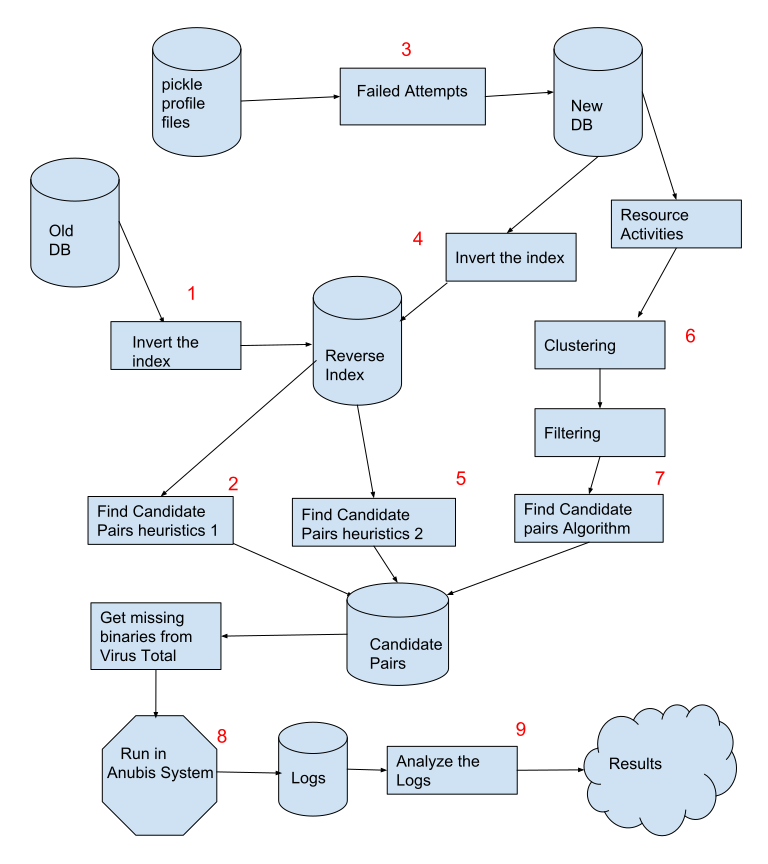
\includegraphics[scale=0.5]{figures/bigpicture.png}
  \caption[Big Picture]{Overview of the research and experiment}\label{fig:bigpicture}
\end{figure}
\section{Candidate Selection}
\label{sec:Candidate Selection}
In this section we illustrate the candidate selection process.
The selection steps are summarized as follows:
\begin{itemize}
  \item Let, \emph{R}, be a set of candidate resources such that each resource ``r'' in \emph{R} have some malware set that create it (say set $A_r$) and some other set of malware that try to (unsuccessfully) access/delete it (say set $B_r$).
  \item Combine all such sets $A_r$ and $B_r$ corresponding to ``r'' in \emph{R} to sets \emph{A} and \emph{B}, respectively.
  \item Combine `A' and `B' and cluster them to cluster ids $[c_1,c_2,\ldots.\ c_n]$ (\emph{n} is number of family) such that any malware sample \emph{x} in (\emph{A} union \emph{B}) can be tagged/mapped to cluster id $C(x)$, where $C(x)$ belongs to $[c_1, c_2, \ldots c_n]$.
  \item For each ``r'' in \emph{R}, generate a set of candidate pairs $p_r$ for experiment. $p_r$ is a set of malware pairs $(x_r, y_r)$ such that $x_r$ belongs to $A_r$ and $y_r$ belongs to $B_r$ and $C(x_r)$ not equal to $C(y_r)$, not belonging to same cluster.
  \item Generate such $(x_r, y_r)$ pairs for all possible cluster pairs $(C(x_r), C(y_r))$ corresponding to a resource ``r''.
  \item The final experiment set \emph{E} is a set of such $(x_r, y_r)$ for all resources \emph{r} in \emph{R}.
  \item Finally for any resource ``r'', if the size of the set $| C(x) : x \in A_r | > 10 or  | C(x) : x \in B_r | > 10$, we discard \emph{r} and its corresponding experiment pairs from \emph{E}, since the resource created/read by too many families is less interesting.
  \item Here $(x,y)$ and $(y,x)$ will be different experiments because we run one sample, wait, and run another sample. Result can be different based on which one runs first. In rare case, both samples may be trying to detect each other.
\end{itemize}
\section{Summary}
\label{sec:Summary}
In this chapter, we described different terms used in our work in details and also gave an overview of our work flow.
In next chapter, we will show how we implemented the work flow in our system.

